\chapter{Going beyond the GDPR -- Exploring the Data Governance Act}
\label{chap:dga}

\begin{tcolorbox}[colback=royallavender!40]
The content of this Chapter has already been partially included in the articles published during this Thesis \citep{esteves_semantifying_2022,esteves_semantics_2023,esteves_towards_2023}.
\end{tcolorbox}

\begin{tcolorbox}[colback=royallavender!10]
The source code produced during the development of this chapter is stored at:
\begin{itemize}
    \item \url{https://w3id.org/dgaterms/repo}
    \item \url{https://w3id.org/people/besteves/soda/repo}
\end{itemize}
\end{tcolorbox}

After witnessing the influence of the GDPR on managing the personal data of European citizens, the European Commission has shifted its attention to establishing a unified data strategy.
This strategy aims to encourage the (re)use and exchange of data among citizens, businesses, and governments, all while ensuring control remains with the original data generators \citep{european_commission_communication_2020}.
In this context, a new series of regulations concerning the usage and management of data is currently under consideration for adoption across the EU countries.
Within this framework, the Data Governance Act (DGA) \citeyearpar{noauthor_regulation_2022}, a regulation primarily focused on regulating the operations of data intermediation services and data altruism organisations, was approved by the Commission in May 2022 and is now mandated for implementation in all EU member states.

This Chapter outlines a range of requirements outlined by the DGA aimed at safeguarding the interests of both data subjects and data holders -- a new legal role inserted in the DGA to refer to entities providing non-personal data --, as well as regulating the jurisdiction of relevant authorities. 
Additionally, it presents various scenarios where the application of Semantic Web technologies, such as the developed work on OAC, ODRL, and DPV, could assist these stakeholders in meeting their respective new rights and responsibilities.
More specifically, it aims to achieve three main goals: (i) generating machine-readable policies for the reuse of public data, (ii) defining consent and permission terms for data altruism, and (iii) establishing standardised registers of data altruism organisations and intermediation service providers and records of their activities.
By leveraging these semantic vocabularies, the aim is not only to enhance machine-readability and interoperability but also to streamline the modelling of data-sharing policies and consent forms across various scenarios, as well as facilitating the creation of a shared semantic framework for maintaining public registers of data intermediaries and altruism organisations, along with documenting their activities.
Given the accessibility and extensibility of these vocabularies, adapting them to meet specific requirements outlined in the DGA becomes a straightforward task.

Section~\ref{sec:dga_flows} provides a description of the DGA and the entities within it, as well as the identification of flows of information between entities.
Moreover, three scenarios where Semantic Web technologies can be leveraged to assist data subjects and data holders in establishing the conditions for the reuse of their data, and public sector bodies, data intermediaries and altruistic organisations in fulfilling their DGA-related obligations. 

Section~\ref{sec:extending_dga} discusses the usage of ODRL, DPV, DCAT and  other vocabularies to express policies for the reuse and sharing of public sector body-held data, to represent registers of entities and logs of their activities, and to create uniform data altruism forms to record consent actions of data subjects and permissions of data holders.

Section~\ref{sec:soda} describes the development of a Solid Data Altruism application, to implement data altruism as a service using Solid and ODRL policies to grant access to personal data for altruistic purposes in a privacy-friendly manner.

To conclude, Section~\ref{sec:lessons} debates the advantages and challenges of the proposed semantic model towards having semantic interoperability to support the development of common European data spaces.

\section{Information flows in the DGA}
\label{sec:dga_flows}

Figure of information flows and documents (from the paper)
Comparison with GDPR flows
Identification of important use cases that can be tackled and easily extended with the work already developed for GDPR
\section{DGAterms}
\label{sec:dgaterms}

As an active contributor in the realm of data protection, the Semantic Web community possesses significant potential to aid with the compliance processes that such a legislation involve.
Such potential is based on the opportunities for interoperability that such a Web of Linked Data can support.
In this context, Semantic Web technologies can be utilised:
\begin{itemize}
    \item to model conditions for the reuse of public data;
    \item by data subjects, data holders and data users to declare data access and usage policies in a machine-readable format; and
    \item by organisations and service providers to maintain records of the processing activities.
\end{itemize}

% requirements specification -- ORSD
% vocab implementation details
% Vocabulary publication and maintenance
% vocab evaluation
\section{SoDA -- Solid for Data Altruism}
\label{sec:soda}

This Section features an architecture designed to enable data altruism as a service, utilising the Solid protocol and ODRL policies to facilitate the sharing of personal data for altruistic purposes in a manner that respects data protection principles.
The policies are articulated using OAC and the DGAterms concepts related to data altruism.
Furthermore, we introduce the Solid Data Altruism application, SoDA, which allows (a) individuals to create policies for sharing their personal data for altruistic purposes, (b) data users to request access to datasets for altruistic purposes, and (c) data altruism organisations to manage metadata concerning available datasets.

\subsection{Solid architecture for data altruism}
\label{sec:architecture_soda}

The diagram presented in Figure~\ref{fig:soda_architecture} provides a broad summary of an architecture designed to implement data altruism as a service through the usage of the Solid protocol, with the central component being a Solid for Data Altruism application, known as SoDA.
The objective of this architecture is to start a proof of concept decentralised ecosystem for data altruism, emphasising the capability of data subjects to share personal data and data users to discover available datasets suitable for altruistic purposes, in line with data protection principles in the EU as the information disclosed about each dataset is limited to its data type and the intended purpose for its utilisation.

\begin{figure}[ht]
  \centering
  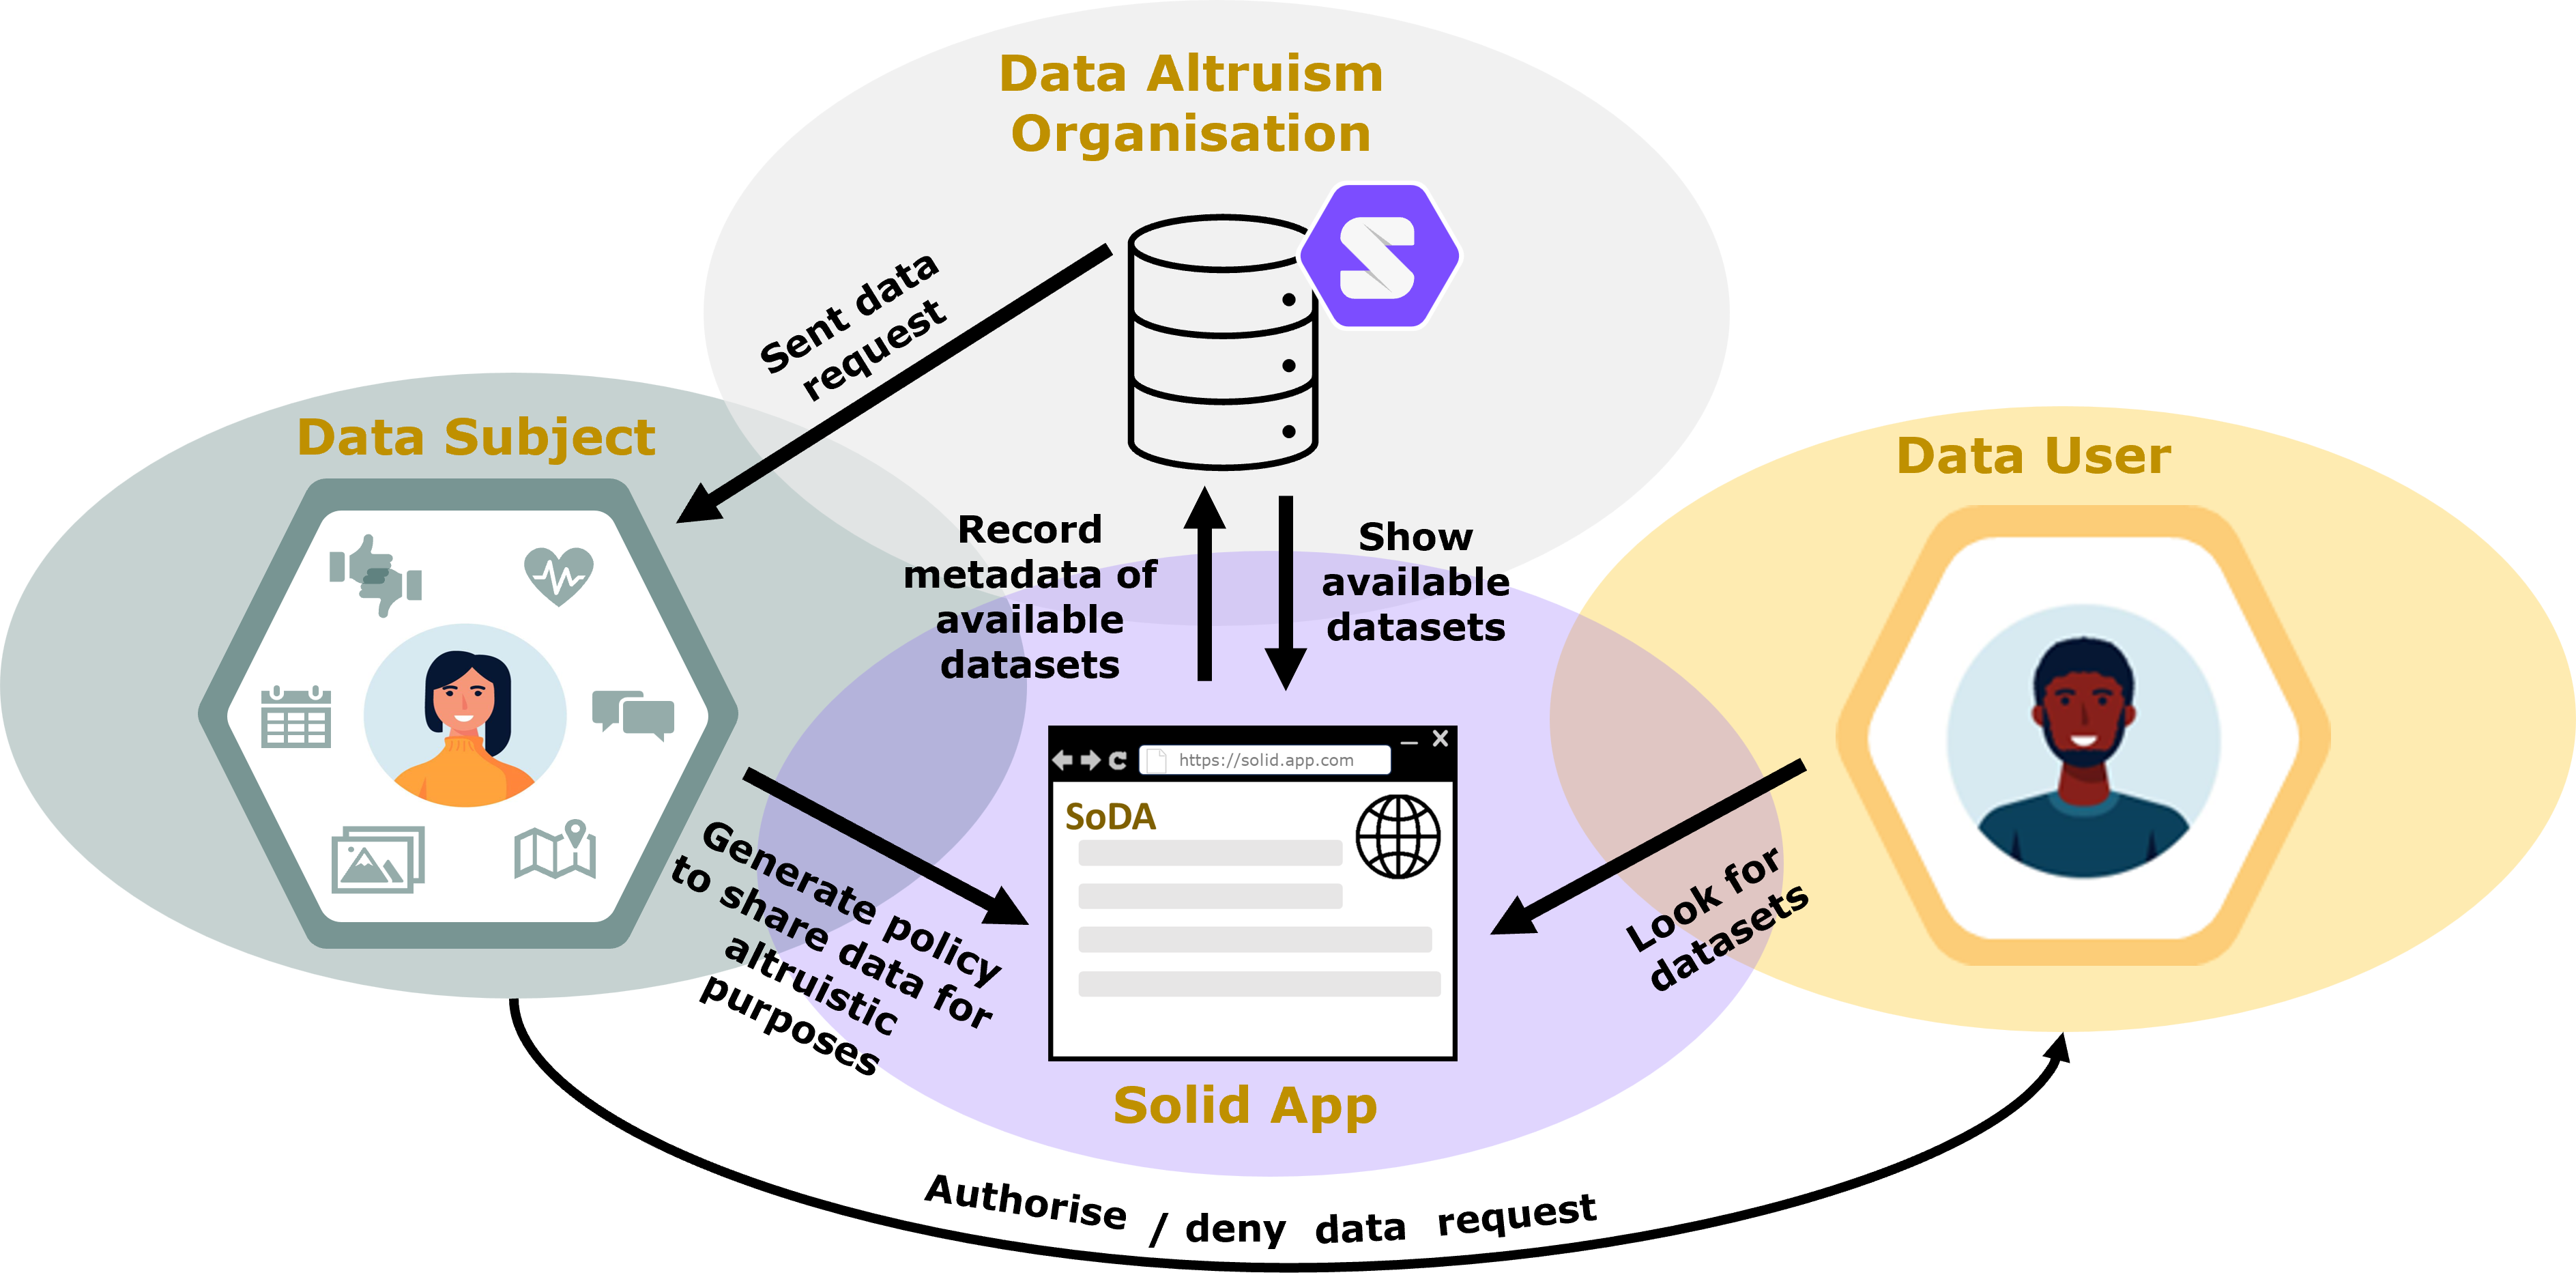
\includegraphics[width=\linewidth]{figures/chapter-7/architecture.png}
  \caption{High-level diagram speifying an architecture to implement data altruism as a service using Solid and SoDA, a Solid application to edit policies/search for data for altruistic purposes, adapted from \cite{esteves_towards_2023}.}
  \label{fig:soda_architecture}
\end{figure}

As previously described, within a Solid-based architecture, users are recognised through a WebID and utilise Solid Pods to either store data or request access to stored data, adhering to the specifications outlined in the Solid protocol.
When personal data resides within Pods, GDPR and DGA requirements come into effect, with individuals who store their personal data in Pods being categorised as `data subjects'.
Additionally, both data subjects and data users administer data access via Solid applications.
In this setting, the SoDA application is introduced to:

\begin{enumerate}
    \item [(a)] empower data subjects to create policies for sharing their personal data with altruistic intent;
    \item [(b)] enable users to seek access to datasets based on their data type and intended purpose for usage; and
    \item [(c)] facilitate organisations in offering data altruism services by maintaining metadata about accessible datasets within their own Solid Pod, without the necessity of storing the data themselves, aligning with Solid's decentralised principles.
\end{enumerate}

With SoDA, individuals can craft data access policies governing their personal data, which are stored in their Solid Pod and can be shared with a data altruism organisation, which exclusively records metadata about the dataset and access conditions.
These records are leveraged to present available datasets to data users, safeguarding the privacy of data subjects by revealing solely the data type and permissible purpose of use, while concealing their identity. 
Should users identify datasets of interest, the data altruism organisation serves as an intermediary, forwarding data requests to the data subjects for them to authorise or deny access to the requested data.
Policies are modelled using OAC -- and by consequence, ODRL and DPV --, and DGAterms, and the catalogues of datasets kept by the altruistic company are based on DCAT.
Detailed instructions on how to install, launch, and use SoDA are available on the source code repository\footnote{\url{https://w3id.org/people/besteves/soda/repo}}.
Figures~\ref{fig:soda-ds} and~\ref{fig:soda-du} present a screenshot of SoDA's (i) policy editor UI and (ii) dataset request UI, respectively.

\begin{figure}[ht]
    \centering
    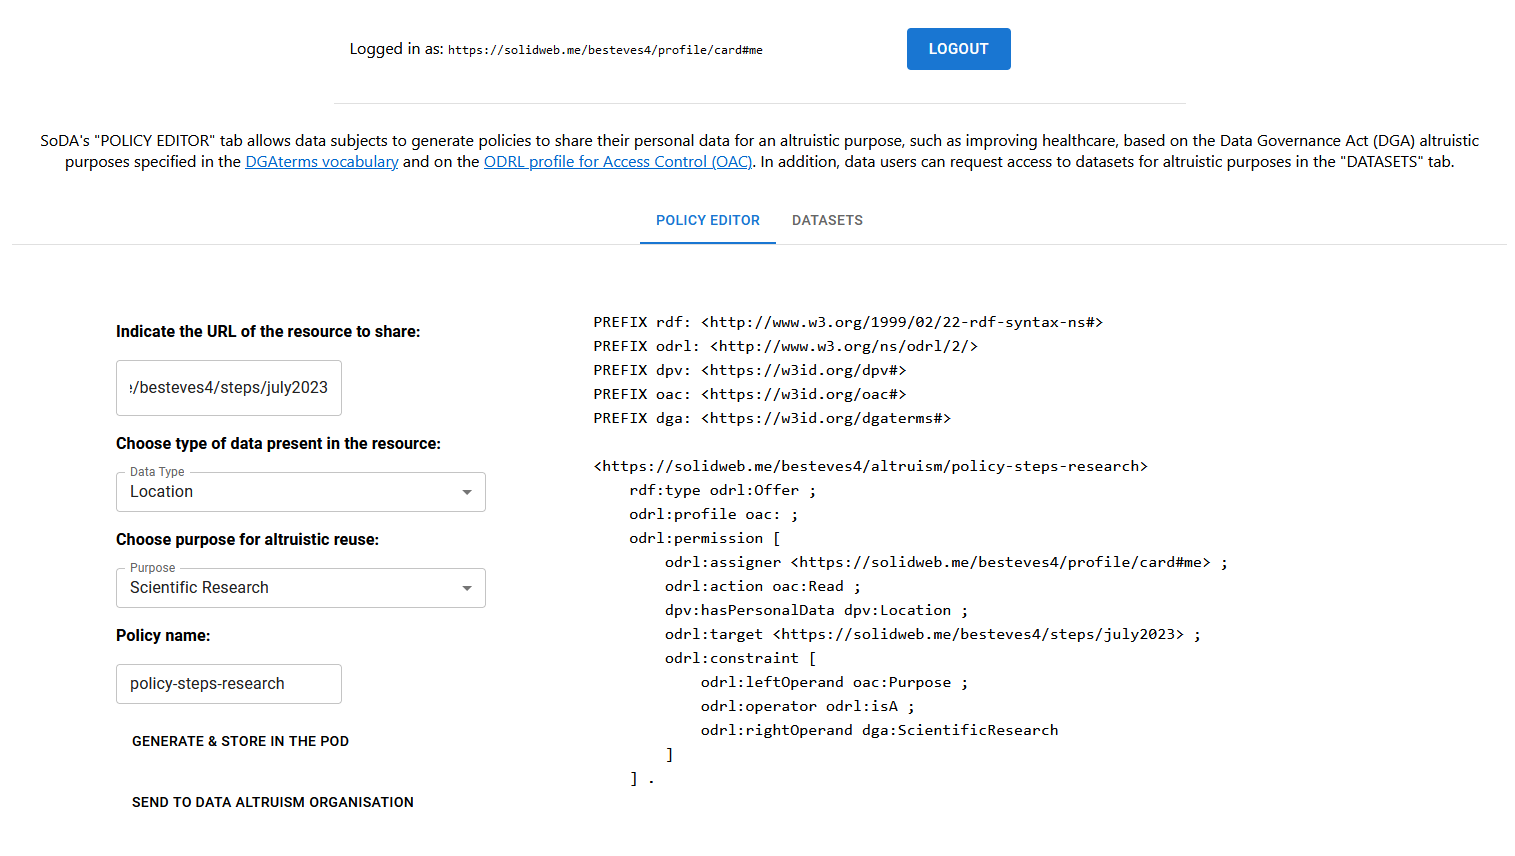
\includegraphics[width=\linewidth]{figures/chapter-7/policy-editor.png}
    \caption{Screenshot of SoDA policy editor UI, which generates OAC and DGAterms-based policies.}
    \label{fig:soda-ds}
\end{figure}

\begin{figure}[ht]
    \centering
    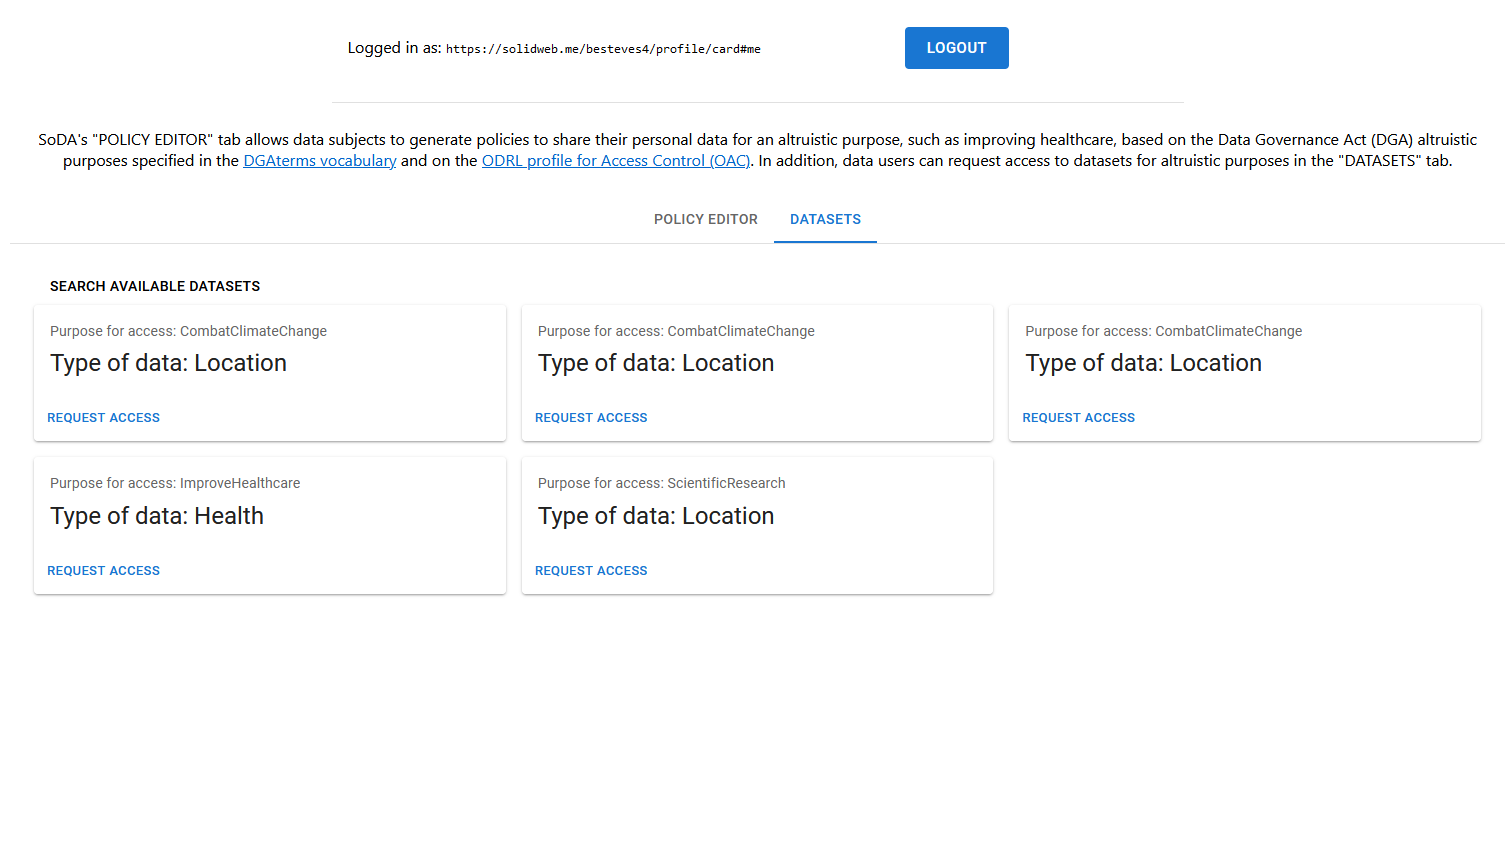
\includegraphics[width=\linewidth]{figures/chapter-7/datasets.png}
    \caption{Screenshot of SoDA dataset request UI, which allows data users to request access to a dataset for a specific purpose.}
    \label{fig:soda-du}
\end{figure}

\subsection{SoDA coverage, maintenance, and future work}
\label{sec:maintenance_soda}

SoDA is published and archived according to the methodology described in Section~\ref{sec:code_preservation}.
Furthermore, SoDA's source code is hosted at \url{https://w3id.org/people/besteves/soda/repo}, under the CC-BY-4.0 license.
Further information on this proof of concept application can be found at \url{https://w3id.org/people/besteves/demo/iswc23}, including a demonstration of the features of the app.
The repository can also be used by SoDA users to suggest new features to be added to the app and to report bugs through GitHub Issues.
Currently, SoDA's app coverage encloses terms from OAC/DPV taxonomies of purposes and personal data categories, focusing on the altruistic purposes described in the DGA.
As future work, SoDA can be extended to include all terms present in the previously mentioned DPV's data taxonomies, as well as to cover all constraints defined in the OAC profile, e.g., restrict legal bases, recipients or specify the technical and organisational measures used by data controllers to ensure the secure processing of personal data.
Additionally, user studies should be performed to assess the design choices included in the policy editor and dataset request UI, as well as to understand what type of additional controls people want to have on top of what is legally mandated, in particular, related to sharing data for altruistic purposes, e.g., temporal constraints or duties for the data user to fulfil after accessing the data.
\section{Lessons learned for the (Personal) Data Spaces future}
\label{sec:lessons}

While the European data strategy is robust, it presents numerous interoperability challenges that must be overcome to establish shared data spaces across individuals, businesses, and governments.
Consequently, the work developed in this Chapter, focusing on analysing the requirements of the DGA and developing a unified semantic model for documenting the activities of public sector bodies, intermediaries, and altruistic organisations, represent an initial stride towards addressing these interoperability hurdles.
In this context, semantic technologies offer promising applications in operationalising compliance with the DGA.
Among them, the following advantages can be mentioned:
\begin{itemize}
    \item \textbf{Enhanced Interoperability} -- Semantic technologies enable better integration and interoperability of data coming from distinct sources and systems, facilitating the work of data altruism organisations and intermediation providers in consolidating datasets coming from different data subjects and other data holders.
    \item \textbf{Improved Knowledge Management} -- By structuring, organising and publishing data with semantic standards, e.g., DCAT for cataloguing datasets, data discovery and analysis can be performed more efficiently.
    \item \textbf{Enhanced Decision Support} -- Semantic technologies enable the development of Web agents with sophisticated decision support systems that can provide actionable insights to data subjects and data holders, aiding them in making informed decisions when it comes to the use of their data.
    \item \textbf{Improved Legal Support} -- Using a common semantic model to tackle legal requirements from distinct data-related regulations, e.g., DPV, aids businesses to have a shared understanding of regulatory provisions and to comply with their legal duties related to the processing of personal and non-personal data.
\end{itemize}

While these advantages are promising, it should be acknowledged that there are challenges that need to be addressed to support the sustainable development of data altruism and data intermediation services towards having common European data spaces:

\begin{itemize}
    \item Most constraints specified in the policies cannot be automatically enforced, and the declarative nature of the policies may inadvertently result in data misuse.
    \item If an agreement is not reached in terms of which semantic models need to be used, interoperability will be difficult to achieve among data subjects, holders, users and even public authorities.
\end{itemize}

As future contributions, it is imperative to explore the potential of the Data Act and the European Health Data Space proposals to enhance the outreach of DPV and achieve the envisioned interoperability to have common European data spaces.
Moreover, to complement the described system, future efforts should include:
(i) implementing SHACL shapes to validate data reuse and data altruism policies,
(ii) conducting usability tests to evaluate the design choices made in SoDA, including scalability testing, which may involve utilising data aggregators to manage organisations seeking simultaneous access to numerous datasets,
(iii) enhancing/automating the process of authorising/denying data requests through technologies such as RDF surfaces \citep{hochstenbach_rdf_2023} to perform reasoning tasks over data policies, and 
(iv) facilitating the creation of immutable agreements, e.g., by integrating Verifiable Credentials into the Solid ecosystem \citep{braun_attributebased_2022} to digitally sign data usage conditions, which can be utilised by authorities in case of misuse by data users.